\documentclass[12pt,letterpaper]{article}

\def\myauthor{John~O.~``Juno''~Woods}
\def\mytitle{jow-vita}
\def\myemail{john.o.woods@gmail.com}
\def\myweb{johnowoods}
\def\myphone{703-801-2625}
\def\mykeywords{
  juno woods
  john woods,
  john o woods,
  john o juno woods
  john oates woods,
  resume, 
  curriculum, 
  vita, 
  curriculum vita, 
  cv, 
  john, 
  woods, 
  jow
}

\setlength\parindent{0pt}

\newenvironment{itemize*}%
{\begin{itemize}%
  \setlength{\itemsep}{0pt}}%
{\end{itemize}}

\usepackage{graphicx}
\usepackage{wrapfig}
\usepackage{pgfplots}
\usepackage{amsmath}
\usepackage{textcomp}
\usepackage{url}
\usepackage{fancyhdr}
\usepackage{lastpage}
%\usepackage{ocgtools}
\usepackage{enumitem}
\setlist{nolistsep,leftmargin=0.15in}
\usepackage[log-declarations=false]{xparse}
%\usepackage{mathdesign}
%\usepackage[no-math]{fontspec}
\usepackage{microtype}
\usepackage[margin=1.125in,top=1.375in,right=1in,left=2in]{geometry}
\usepackage[strict]{changepage}
\usepackage[
  ocgcolorlinks,
  urlcolor={[rgb]{0,0,0.54}},
  unicode,
  plainpages=false,
  pdfpagelabels,
  pdftitle={\mytitle},
  pdfauthor={\myauthor},
  pdfkeywords={\mykeywords}
]{hyperref}
\usepackage{relsize}

% Use sans serif fonts in plot
\usepackage[eulergreek]{sansmath}
\pgfplotsset{
  every axis/.append style = {font=\sansmath\sffamily},
  %every axis label = {font=\sansmath\sffamily},
  %legend style = {font=\sansmath\sffamily},
  %tick label style = {font=\sansmath\sffamily},
  %every node style = {font=\sansmath\sffamily}
  }

% fix ocgcolor link breaking; thanks due to Benjamin Lerner (http://goo.gl/VZKR7M)
\makeatletter
\AtBeginDocument{%
  \newlength{\temp@x}%
  \newlength{\temp@y}%
  \newlength{\temp@w}%
  \newlength{\temp@h}%
  \def\my@coords#1#2#3#4{%
    \setlength{\temp@x}{#1}%
    \setlength{\temp@y}{#2}%
    \setlength{\temp@w}{#3}%
    \setlength{\temp@h}{#4}%
    \adjustlengths{}%
    \my@pdfliteral{\strip@pt\temp@x\space\strip@pt\temp@y\space\strip@pt\temp@w\space\strip@pt\temp@h\space re}}%
  \ifpdf
    \typeout{In PDF mode}%
    \def\my@pdfliteral#1{\pdfliteral page{#1}}% I don't know why % this command...
    \def\adjustlengths{}%
  \fi
  \ifxetex
    \def\my@pdfliteral #1{\special{pdf: literal direct #1}}% isn't equivalent to this one
    \def\adjustlengths{\setlength{\temp@h}{-\temp@h}\addtolength{\temp@y}{1in}\addtolength{\temp@x}{-1in}}%
  \fi%
  \def\Hy@colorlink#1{%
    \begingroup
      \ifHy@ocgcolorlinks
        \def\Hy@ocgcolor{#1}%
        \my@pdfliteral{q}%
        \my@pdfliteral{7 Tr}% Set text mode to clipping-only
      \else
        \HyColor@UseColor#1%
      \fi
  }%
  \def\Hy@endcolorlink{%
    \ifHy@ocgcolorlinks%
      \my@pdfliteral{/OC/OCPrint BDC}%
      \my@coords{0pt}{0pt}{\pdfpagewidth}{\pdfpageheight}%
      \my@pdfliteral{F}% Fill clipping path (the url's text) with current color
      \my@pdfliteral{EMC/OC/OCView BDC}%
      \begingroup%
        \expandafter\HyColor@UseColor\Hy@ocgcolor%
        \my@coords{0pt}{0pt}{\pdfpagewidth}{\pdfpageheight}%
        \my@pdfliteral{F}% Fill clipping path (the url's text) with \Hy@ocgcolor
      \endgroup%
      \my@pdfliteral{EMC}%
      \my@pdfliteral{0 Tr}% Reset text to normal mode
      \my@pdfliteral{Q}%
    \fi
    \endgroup
  }%
}
\makeatother
% end fixes


\newcommand{\Cpp}{\textsc{c}\nolinebreak[4]\hspace{-.05em}\raisebox{.4ex}{\relsize{-3}{\textbf{++}}}}
\newcommand{\Magickpp}{Magick\nolinebreak[4]\hspace{-.05em}\raisebox{.4ex}{\relsize{-3}{\textbf{++}}}}
\newcommand{\Star}{\textsc{Star-CCM\ensuremath{+}}}

\newcommand{\mhead}[1]{\leavevmode\marginpar{\sffamily\footnotesize #1}}
%\newcommand{\rdate}[1]{{\addfontfeature{Numbers=OldStyle} \hfill #1}}
%\renewcommand{\date}[1]{{\addfontfeature{Numbers=OldStyle} #1}}
\newcommand{\rdate}[1]{{\hfill #1}}
\renewcommand{\date}[1]{{#1}}
\renewcommand{\labelitemi}{-} 

%\setmainfont[
%  Ligatures={TeX,Common},
%  BoldFont={AGaramondPro-Semibold},
%]{Adobe Garamond Pro}
%\setsansfont[
%  Ligatures={TeX,Common},
%  Letters=SmallCaps,
%  Color=660000,
%]{Adobe Garamond Pro}
%\setmonofont[Scale=0.85]{FontAwesome}

%\makeatletter % fix for \hrulefill w/ mathdesign package
%\def\hrulefill{\leavevmode\leaders \hrule height \rulethickness \hfill\kern\z@}
%\makeatletter

\begin{document}\flushbottom
\pagestyle{fancy} \setlength\headwidth{6.5in}
\rhead{\textsc{Dr.~John~O.~``Juno''~Woods --- curriculum vitae --- \thepage{} of \pageref*{LastPage}}} \cfoot{}
\thispagestyle{empty}
\begin{adjustwidth}{-1in}{}
{\Huge
  {\textsc{%
    {%\addfontfeature{Style=TitlingCaps}
    J}\kern-1.0ptohn 
    {%\addfontfeature{Style=TitlingCaps}
    O}\kern-2pt.~``%
    {%\addfontfeature{Style=TitlingCaps}
    J}\kern-2ptuno''~%
    {%\addfontfeature{Style=TitlingCaps}
    W}\kern-2.5ptoods, PhD}
  }
}
%
{
  \begin{minipage}[b]{1.3in}
    \flushleft \footnotesize   
    %Houston, \textsc{tx} \\
    %Oakland, \textsc{ca}
  \end{minipage}
  \hfill
  \begin{minipage}[b]{1.5in}
    \flushright \footnotesize 
    \href{tel:\myphone}{\myphone} \\ %\texttt{}~
    \href{mailto:\myemail}{\myemail} \\
    github:\href{https://github.com/autumnsault}{autumnsault}% \\
    %linkedin:\href{https://www.linkedin.com/in/johnowoods}{‚Œjohnowoods}
  \end{minipage}
}\par
\hrulefill

\centering\small guidance, navigation, \& control\hskip 3mm$\circ$\hskip 3mm computer science\hskip 3mm$\circ$\hskip 3mm mission design \& analysis %evolutionary systems biology
\vskip-6pt
\hrulefill
\end{adjustwidth}  
\reversemarginpar 
\setlength\marginparwidth{0.85in}
\smallskip
\mhead{Education}%
\textbf{The University of Texas at Austin,} Austin, Texas \newline
\emph{Doctor of Philosophy%, Cell \& Molecular Biology (Bioinformatics)} 
}\rdate{2007--2013}
\begin{itemize*}
  \item National Science Foundation Fellow (2009--2012)%, \href{http://cssb.utexas.edu/}{Center for Systems \& Synthetic Biology}
  \item Dissertation: \href{https://www.dropbox.com/s/87v8j47mxo0afgj/diss.pdf}{Predicting gene--phenotype associations in humans and other species from orthologous and paralogous phenotypes}
  \item Advisor: Dr.~Edward~M.~Marcotte
\end{itemize*}

\medskip
\textbf{Virginia Polytechnic Institute \& State University,} Blacksburg, Virginia \newline
\emph{Bachelor of Science, Computer Science}, magna cum laude \rdate{2002--2007}
\begin{itemize*}
  %\item Graduated \emph{magna cum laude}
  \item Minors in Mathematics, Philosophy, and Russian
\end{itemize*}
%
\begin{wrapfigure}{R}{2in}
\vspace{-25pt}%
\centering%
%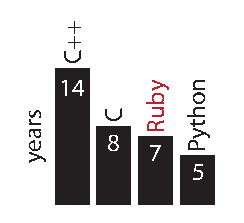
\includegraphics[width=2in]{programming-graph.pdf}%
\begin{tikzpicture}
\begin{axis}[ybar
			, symbolic x coords={C++, C, Ruby, Python, Matlab},
			, ylabel={years}
			, ylabel near ticks
			, ymajorgrids=true
			, axis on top
			, grid style={draw=white, line width=1pt}
			, major tick length=0pt
			, ymin=0
			, xtick=data
			, fill=black
			, fill opacity=1.0
			, draw=white
			, bar width=0.05\textwidth
			, nodes near coords
			, every node near coord/.append style={rotate=90, anchor=west, color=black}
			, width=2in
			, xmajorticks=false
			]
\addplot+[point meta=explicit symbolic,fill=black,draw=white] coordinates {
	(C++,17) [C\footnotesize{++}]
	(C,11) [C]
	(Ruby,10) [Ruby]
	(Python,8) [Python]
	(Matlab,3) [Matlab]
};
\end{axis}
\end{tikzpicture}
\vspace{-15pt}%
\end{wrapfigure}%
%
\bigskip
\mhead{Coding \newline Proficiencies}%
%\emph{Strong}\ 
\textsc{c},
\Cpp\ (including modern extensions),
Ruby,
Python (including \textsc{c} extensions),
\LaTeX,
\textsc{gnu} Octave and \textsc{Matlab},
shell scripting%,

\medskip
\emph{Familiar}\ 
Java, Agile development methodology, Perl,
%\textsc{Fortran}~95,
%Perl,
\textsc{R},
\textsc{sql}

\medskip
\emph{Libraries}\ 
Orekit (Python \textsc{api}),
\textsc{Spice}, SpiceyPy,
Point Cloud Library$^\dagger$,
\textsc{flann}$^\dagger$ ($k$ nearest neighbors),
\Cpp\ \textsc{stl} and Boost,
\textsc{assimp},
ImageMagick/\Magickpp,
%\textsc{atlas},
%\textsc{lapack},
%\textsc{blas},
%\textsc{gnu} Scientific Library,
Open\textsc{gl},
\textsc{glsl},
%\textsc{glm},
Eigen,
\textsc{Trick} simulator,
\textsc{Nm}atrix$^\ddagger$,
Pyquat$^\ddagger$ (Python attitude library),
\textsc{Glidar}$^\ddagger$ (\textsc{3d lidar} simulator),
Starlib$^\ddagger$ (complete rewrite of open source star tracker)

\smallskip
$^\dagger$\,{\footnotesize indicates code contributed to library}\newline
$^\ddagger$\,{\footnotesize indicates primary authorship}

\medskip
\emph{Software}\
Copernicus, 
Git,
%Gnuplot,
%Emacs,
%Vim,
%Bash,
%Zsh,
\textsc{gcc},
Clang,
\textsc{gdb},
Valgrind,
\textsc{cm}ake,
Ubuntu,
Mac \textsc{os\,x}

\bigskip
\mhead{Professional \newline Appointments}%
\vskip -1em
\textbf{Open Lunar Foundation,} San Francisco, California \newline
\emph{Guidance, Navigation, \& Control} \rdate{\textsc{oct}~2019--\textsc{apr}~2020}
\begin{itemize*}
  \item Developed open source linear covariance analysis tool for sensor selection, including horizon-based optical navigation
  \item Orbit determination, radiometric strategy design, and covariance analysis using Orekit
  \item Prototyped $q$-method extended Kalman filter (for attitude)
  \item Supervised graduate student developing an open source tool for generating circular restricted three-body problem cislunar trajectories
  \item Laid off as part of \textsc{covid}-19-related force reduction
\end{itemize*}
  
\medskip
\textbf{Intuitive Machines,} Houston, Texas \newline
\emph{Senior Development Engineer} \rdate{\textsc{jun}~2015--\textsc{oct}~2019}
\begin{itemize*}
  \item Mission and trajectory design --- \textsc{nova-c} lunar lander
  \item Navigation filters and simulation sensor models --- \textsc{Im}'s Terrestrial Return Vehicle / Universal Return Vehicle, Moon Express \textsc{mx}-1
  \item Payload requirements, \textsc{gn\&c} design --- Axiom commercial space station module
  \item Error budget analysis and filter prototype --- aircraft-based gravimetry
  \item Measurement models and filter prototype --- \textsc{Gps}-denied planetary navigation
%  \item Responsible for universal navigation filter in \textsc{im}'s universal flight software, to be flown on a deorbiter (Terrestrial Return Vehicle, or \textsc{trv}) and Moon Express' moon lander; documented and re-derived filter; wrote and validated sensor models in \textsc{nasa} \textsc{trick} physics simulator
%  \item Wrote engineering requirements for payloads and maintained \textsc{gn\&c} requirements for rendezvous and docking of Axiom commercial space station modules with \textsc{iss}; implemented attitude control and targeting algorithms and performed solar power study; created mission design
%  \item Studied cislunar navigation architectures with focus on range dilution of precision
%  \item Designed and implemented multiple dual-state extended Kalman filters and complementary filters for aircraft, spacecraft, and drilling systems
%  \item Performed error budget analysis and designed and prototyped \textsc{ekf} for gravimetry and \textsc{gps}-denied planetary navigation
\end{itemize*}

\bigskip
\mhead{Academic \newline Appointments}%
\textbf{Applied Space Exploration Laboratory,} West Virginia University \newline
\emph{Post-doctoral Fellow --- Aerospace Engineer} \rdate{\textsc{jan}~2014--\textsc{jun}~2015}
\begin{itemize*}
  \item Developed fast, accurate \textsc{lidar}-based \textsc{6\,dof} pose initialization strategy for non-cooperative rendezvous
  \item Derived/implemented dual inertial state \textsc{ekf} with asynchronous measurement updates
  \item Developed open source Open\textsc{gl}-based \textsc{3d} sensor simulator, \textsc{Glidar}
  \item Studied remote sensing technologies for space natural resource surveying and utilization
  \item Mentored and collaborated with grad students and an undergraduate
\end{itemize*}

\medskip
\textbf{Center for Systems \& Synthetic Biology,} The University of Texas at Austin\newline
\emph{National Science Foundation Fellow; Graduate Research Assistant}  \rdate{2007--2014}
\begin{itemize*}
  \item Designed and implemented algorithms and data structures in Python, Perl, Ruby, and \textsc{c}/\Cpp
  %\item Formulated hypotheses relating to an aspect of evolutionary theory called deep homology
  \item Wrote software for automating processing of large data sets and validating hypotheses%, by quickly predicting gene--disease and gene--phenotype associations
  %\item Researched, designed, and wrote statistical software for searching for genes under various types of selection (positive, purifying, relaxed)
  %\item Invalidated a hypothesis about \textsc{hiv} reservoirs using viral evolution simulation
  %\item Designed scheme for re-engineering cellular metabolism in \textit{E.~coli}, and partially implemented it (wet lab)
\end{itemize*}

\medskip
\textbf{Dept. of Chemistry \& Biochemistry,} The University of Texas at Austin\newline
\emph{Graduate Teaching Assistant} \rdate{2008, 2013}
%\begin{itemize*}
%  \item Served as \textsc{ta} for Biochemistry, Introduction to Bioinformatics (graduate level), and Chemistry for non-science majors
%  \item Rewrote curriculum for Introduction to Bioinformatics in Python (previously in Perl)
%\end{itemize*}

\bigskip
\mhead{Community Contributions}
\vskip -1em
\textbf{Black Rock Rangers}\newline
\emph{Ranger} \rdate{2018--\textsc{present}}\newline
\emph{Green Dot} \rdate{2019--\textsc{present}}

%\medskip
%\textbf{Starship Factory}\newline
%\emph{Artist, Organizer} \rdate{2016--2017}%\newline
%\emph{Organizer} \rdate{2017}
%\begin{itemize*}
%  \item Organized artist collective which attempts to envision and bring about a future worth looking forward to
%  \item Created interactive art for Burning Flipside (2017) and Burning Man (2016 and 2017)
%\end{itemize*}

\medskip
\textbf{Ruby Science Foundation (SciRuby)} \newline %The Ruby Science Foundation: The SciRuby Project}\newline
\emph{Director \& Co-Founder} \rdate{2012--\textsc{present}}
%\begin{itemize*}
%  \item Wrote \textsc{Nm}atrix, dense and sparse linear algebra software for Ruby, in \textsc{c}/\Cpp
%  \item Organized the SciRuby Project, dedicated to enhancing the Ruby language's numerical and scientific computing facilities
%  \item Applied for grants, mentored graduate and undergraduate students
%  \item Wrote four successful Google Summer of Code applications and directed mentors
%\end{itemize*}

\medskip
\textbf{Austin Swing Syndicate}\newline
\emph{At-Large Board Member, Secretary} \rdate{2012--2014}%\newline
%\emph{Secretary} \rdate{2013--2014}
%\begin{itemize*}
  %\item Revised bylaws, counseled board on non-profit law and best practices
  %\item Managed teams of volunteers
%  \item Created policy for providing grants to other organizations for events furthering organizational mission of promoting lindy hop, balboa, shag, and other traditional jazz dances
%\end{itemize*}

\medskip
\textbf{Texas Gun Sense}\newline
\emph{Co-founder, Advisory Board Member} \rdate{2013--\textsc{present}}%\newline
%\emph{Advisory Board Member} \rdate{2014--\textsc{present}}
%\begin{itemize*}
%  \item Co-founded an organization promoting a fact-based dialogue around the belief that gun ownership is an individual right, best preserved by ensuring that firearms stay out of the hands of criminals
%  \item Organized and motivated volunteers to testify and lobby at the state level
%  \item Wrote bylaws and 501(c)(3) filing (approved on first attempt)
%  \item Successfully devised legislative strategies to kill bills, two sessions in a row
%  \item Wrote talking points for lawmakers to use in floor debates
%  \item Conferred with legislators and Texas Legislative Council to draft a universal background checks bill
%  \item Served as official spokesperson, including hundreds of interviews (television, radio, film; list available upon request)
%\end{itemize*}

\newpage
%\bigskip
\mhead{Patents}%
\par\vspace{-\baselineskip}Marcotte, E.M.; McGary, K.; Wallingford, J.; Park, T.J.; \textbf{Woods,~J.O.}; Cha,~H.J. 12 August 2012. Orthologous phenotypes and non-obvious human disease models. \textit{U.S.\ Patent Application Publication 2012/0215458 A1}.

\bigskip
\mhead{Articles}%
\par\vspace{-\baselineskip}\textbf{Woods, J.O.}; Christian, J.A. 2016. \textsc{Lidar}-based relative navigation with respect to non-cooperative objects. \textit{Acta Astronautica 126}: pp.\ 298--311.

\medskip
\par\textbf{Woods, J.O.}; Christian, J.A. 2016. \textsc{Glidar}: An OpenGL-based, real-time, and open source 3\textsc{d} sensor simulator for testing computer vision algorithms. \textit{Journal of Imaging 2}(1).

\medskip
\par\textbf{Woods, J.O.}; Tien, M.Z.; Marcotte, E.M. April 2015. Interrogating conserved elements of diseases using Boolean combinations of orthologous phenotypes. \textit{BioR$\chi$iv}.

\medskip
\par\textbf{Woods, J.O.}; Singh-Blom, U.M.; Laurent, J.M.; McGary, K.L.; Marcotte, E.M. January 2013. Prediction of gene--phenotype associations in humans, mice, and plants using phenologs. \textit{BMC Bioinformatics 14}: p.\ 203.

\medskip
\par Singh-Blom, U.M.; Natarajan, N.; Tewari, A.; \textbf{Woods, J.O.}; Dhillon, I.S.; Marcotte, E.M. January 2013. Prediction and validation of gene--disease associations using methods inspired by social network analyses. \textit{PLoS One 8}(5): e58977.

\medskip
\par McGary, K.L.; Park, T.J.; \textbf{Woods, J.O.}; Cha, H.J.; Wallingford, J.B.; Marcotte, E.M. April 2010. Systematic discovery of nonobvious human disease models through orthologous phenotypes. \textit{Proceedings of the National Academy of Sciences of the United States of America 107}(14): pp.\ 6544--9.

\medskip
\par Brennan, T.P.; \textbf{Woods, J.O.}; Sedaghat, A.R.; Siliciano, J.D.; Siliciano, R.F.; Wilke, C.O. September 2009. Analysis of human immunodeficiency virus type 1 viremia and provirus in resting $\textsc{cd4}^{+}$ \textsc{t} cells reveals a novel source of residual viremia in patients on antiretroviral therapy. \textit{Journal of Virology 83}(17): pp.\ 8470--81.

\bigskip
\mhead{Conference \newline Proceedings}%
\par\vspace{-\baselineskip}\textbf{Woods, J.O.}; Christian, J.A.; Evans, T. February 2015. A \textsc{6-dof} pose initialization strategy for \textsc{lidar}-based non-cooperative navigation. In \textit{38th Annual Guidance \& Control Conference}, Breckenridge, CO.

\medskip
Sell, J.L.; Rhodes, A.; \textbf{Woods, J.O.}; Christian, J.A.; Evans, T. 2014. In \textit{AIAA/AAS Astrodynamics Specialist Conference}, San Diego, CA.

\bigskip
\mhead{Posters}%
\par\vspace{-\baselineskip}\textbf{Woods, J.O.}; Singh-Blom, U.M.; Laurent, J.; McGary, K.L.; Marcotte, E.M. 20--25 February 2012. In \textit{Complex Traits: Genomics and Computational Approaches}, Keystone Symposia, Breckenridge, CO.

\medskip
\par \textbf{Woods, J.O.}; Singh-Blom, U.M.; McGary, K.L.; Marcotte, E.M. 13--16 November 2010. In \textit{From Functional Genomics to Systems Biology},  EMBL Heidelberg, Heidelberg, Germany.
\newpage
\mhead{Technical \newline Reports}%
\par\vspace{-\baselineskip}\textit{Some internal technical report titles have been changed for external clarity or to maintain client confidentiality.}

\medskip
\par\textbf{Woods, J.O.} 2019. Navigation filter design towards a lunar lander. \textit{OLF--GNC--2019--02}, Open Lunar Foundation, San Francisco, CA. \textit{Work in progress, ceased and published early due to pandemic.} \href{https://github.com/openlunar/navmemos/raw/master/filter/filter.pdf}{github.com/openlunar/navmemos/ raw/master/filter/filter.pdf}

\medskip
\par\textbf{Woods, J.O.} 2019. Two-way range and range-rate observables in a sequential filter. \textit{OLF--GNC--2019--01}, Open Lunar Foundation, San Francisco, CA. \href{https://github.com/openlunar/navmemos/raw/master/radiometric/memo.pdf}{github.com/openlunar/navmemos/raw/master/radiometric/memo.pdf}

\medskip
\par\textbf{Woods, J.O.} 2018. Observability and sensitivity analyses for attitude estimation using a gimballed gyroscope. \textit{IM--TM--2018--04}.

\medskip
\par \textbf{Woods, J.O.} 2018. Position and velocity variance growth during dead reckoning of a drill. \textit{IM--TM--2018--02}.

\medskip
\par \textbf{Woods, J.O.} 2018. Derivation of the Doppler \textsc{lidar} measurement model in the inertial and topocentric frames. \textit{IM--TM--2018--01}.

\medskip
\par Crain, T.C.; \textbf{Woods, J.O.}; Baine, M.; Moore, J.; Getchius, J.; Ronalds, A.; Stewart, S. 2018. Cislunar navigation architecture study. \textit{IMDM--9}.

\medskip
\par \textbf{Woods, J.O.} 2017. A dual \textsc{marg} complementary filter for attitude state estimation while drilling. \textit{IM--TM--2017--04}.

\medskip
\par \textbf{Woods, J.O.}; Christian, J.A. 2014. A real-time, software-based \textsc{3d} sensor simulator. ASEL Technical Memorandum: \textit{ASEL--14--005}.

\medskip
\par Sell, J.; Rhodes, A.; \textbf{Woods, J.}; Christian, J.A. 2014. Theoretical foundations of pose estimation and covariance computation for non-cooperative relative navigation. ASEL Technical Memorandum: \textit{ASEL--14--001}.

\medskip
\par Natarajan, N.; Singh-Blom, U.M.; Tewari, A.; \textbf{Woods, J.O.}; Dhillon, I.S.; Marcotte, E.M. 2011. Predicting gene--disease associations using multiple species data. UTCS Technical Report: \textit{TR--11--37}.


%\bigskip
%\mhead{Invited Talks}%
%\par\vspace{-\baselineskip}\textsc{Sxsw}edu session: Keeping Schools Secure. 11 March 2015.
%
%\medskip
%\par Texas Conference on School-Based Law Enforcement: Panel Discussion. 2010.

\bigskip
\mhead{Honors \& \newline Awards}%
Paul Harris Fellowship                                              \rdate{2018}\newline
Necklace Factory / Burning Man Art Award                            \rdate{2016}\newline
White House Champion of Change (Obama Administration)				\rdate{2014}\newline
National Science Foundation Graduate Research Fellowship			\rdate{2009--2012}\newline
``Best of Austin'' Award: Best Activist	(\emph{The Austin Chronicle})							\rdate{2011}\newline
Scholar, Netroots Nation											\rdate{2011}\newline
Initiate, Friar Society (University of Texas at Austin)				\rdate{2010}\newline
Graduate School Recruitment Fellowship (University of Texas at Austin) \rdate{2007}\newline
Black Belt, Tae Kwon Do (Chung Do Kwan)								\rdate{2006}\newline
Member, Hillcrest Honors Community (Virginia Tech)				\rdate{2003--2007}\newline
Inductee, $\Upsilon\Pi\mathrm{E}$ (Virginia Tech)					\rdate{2006}\newline
Gilbert \& Lucille Seay Scholarship (Virginia Tech)					\rdate{2005}\newline
National Merit Scholarship											\rdate{2002}\newline

\bigskip
\mhead{Media}%
\par\vspace{-\baselineskip}\textit{Media appearances available upon request.}

\bigskip
\mhead{Activities \& \newline Interests}%
dance (lindy hop and ballet),
circus arts,
space exploration,
large-scale interactive art

\bigskip
\mhead{Foreign\newline Languages}%
English (native tongue), 
Spanish (conversational), 
Russian (needs refreshing),
Mandarin (learning)\newline
%French, German, Mandarin (smattering)

\bigskip
\mhead{References}%
John~Christian\rdate{\href{mailto:john.christian@mail.wvu.edu}{john.christian@mail.wvu.edu}}\newline
Asst.\ Professor of Aerospace Engineering, Rensselaer Polytechnic Institute

\medskip
Tim~Crain\rdate{\href{mailto:tim@intuitivemachines.com}{tim@intuitivemachines.com}}\newline
Vice President of Research and Development, Intuitive Machines

\medskip
Amanda~Acevedo\rdate{\href{mailto:amanda.acevedo@vedosystems.com}{amanda.acevedo@vedosystems.com}}\newline
President, Vedo Systems; formerly Project Manager, Intuitive Machines

\medskip
Chris~Hadfield\rdate{\href{mailto:chris@chrishadfield.ca}{chris@chrishadfield.ca}}\newline
Chair, Open Lunar Foundation; Commander, \textsc{csa} and \textsc{nasa}

\medskip
Ben~Howard\rdate{\href{mailto:ben@openlunar.org}{ben@openlunar.org}}\newline
Chief Engineer, Open Lunar Foundation; Chief Spacecraft Architect, Planet

%\medskip
%Edward~Marcotte\rdate{\href{mailto:marcotte@icmb.utexas.edu}{marcotte@icmb.utexas.edu}\hskip 0.5cm\href{tel:512-471-5435}{512-471-5435}}\newline
%Professor of Chemistry \& Biochemistry, The University of Texas at Austin


\end{document}